%%%%%%%%%%%%%%%%%%%%%%%%%%%%%%%%%%%%%%
% LaTeX poster template
% Created by Nathaniel Johnston
% August 2009
% http://www.nathanieljohnston.com/2009/08/latex-poster-template/
%%%%%%%%%%%%%%%%%%%%%%%%%%%%%%%%%%%%%%

\documentclass[final]{beamer}
\usepackage[scale=1.24]{beamerposter}
\usepackage{graphicx}			% allows us to import images

%-----------------------------------------------------------
% Define the column width and poster size
% To set effective sepwid, onecolwid and twocolwid values, first choose how many columns you want and how much separation you want between columns
% The separation I chose is 0.024 and I want 4 columns
% Then set onecolwid to be (1-(4+1)*0.024)/4 = 0.22
% Set twocolwid to be 2*onecolwid + sepwid = 0.464
%-----------------------------------------------------------

\newlength{\sepwid}
\newlength{\onecolwid}
\newlength{\twocolwid}
\newlength{\threecolwid}
\setlength{\paperwidth}{48in}
\setlength{\paperheight}{36in}
\setlength{\sepwid}{0.024\paperwidth}
\setlength{\onecolwid}{0.22\paperwidth}
\setlength{\twocolwid}{0.464\paperwidth}
\setlength{\threecolwid}{0.708\paperwidth}
\setlength{\topmargin}{-0.5in}
\usetheme{confposter}
\usepackage{exscale}

%-----------------------------------------------------------
% The next part fixes a problem with figure numbering. Thanks Nishan!
% When including a figure in your poster, be sure that the commands are typed in the following order:
% \begin{figure}
% \includegraphics[...]{...}
% \caption{...}
% \end{figure}
% That is, put the \caption after the \includegraphics
%-----------------------------------------------------------

\usecaptiontemplate{
\small
\structure{\insertcaptionname~\insertcaptionnumber:}
\insertcaption}

%-----------------------------------------------------------
% Define colours (see beamerthemeconfposter.sty to change these colour definitions)
%-----------------------------------------------------------

\setbeamercolor{block title}{fg=ngreen,bg=white}
\setbeamercolor{block body}{fg=black,bg=white}
\setbeamercolor{block alerted title}{fg=white,bg=dblue!70}
\setbeamercolor{block alerted body}{fg=black,bg=dblue!10}

%-----------------------------------------------------------
% Name and authors of poster/paper/research
%-----------------------------------------------------------

\title{Punitive Measures: Because Finding a Good Pun is its own Reword}
\author{GROUP C - Amir Kashipazha, Brandon Boylan-Peck, Cathlyn Stone, Kenneth Hunter Wapman, Shantanu Karnwal}
\institute{CSCI 5622 (Machine Learning), University of Colorado Boulder}

%-----------------------------------------------------------
% Start the poster itself
%-----------------------------------------------------------

\begin{document}
\begin{frame}[t]
	\begin{columns}[t] % the [t] option aligns the column's content at the top
		%----------------------------------------------------------------------------------------
		\begin{column}{\sepwid}\end{column}
		%----------------------------------------------------------------------------------------
		\begin{column}{\onecolwid}

			\vspace{110mm}
			\begin{block}{Puns}
				{\large
					A \textbf{Pun} is form of wordplay in which a word\textquotesingle s multiple meanings or similar sounding words are used in a comedical manner. \\
					\vspace{40mm}
					Accurate identification and interpretation of puns would help improve human-computer communication, machine translation, and literary analysis.\\
					\vspace{40mm}
					There are many types of puns, but we focused on these two types:\\
						\\
					
					\begin{itemize}
						\item {\textbf{Homographic}: A pun involving two words whose spellings are the same but have different meanings.\\
								\textit{I used to be a banker but I lost \textbf{interest}.}}
						\item {\textbf{Heterographic}: A pun involves two or more words which sound alike but are spelled differently.\\
								\textit{Two construction workers had a \textbf{stairing} contest.}}
					\end{itemize}
					\vspace{40mm}
					We worked on two tasks: 
					\begin{itemize}
						\item {Pun \textbf{Detection}: determining whether a sentence is a pun or not}
						\item {Pun \textbf{Location}: identifying the word in a pun sentence which `makes' the pun}
					\end{itemize}
				}
			\end{block}
		\end{column}
		%----------------------------------------------------------------------------------------
		\begin{column}{\sepwid}\end{column}
		%----------------------------------------------------------------------------------------
		% center column (tasks)
		%----------------------------------------------------------------------------------------
		\begin{column}{\twocolwid}
			%----------------------------------------------------------------------------------------
			% top row
			%----------------------------------------------------------------------------------------
			\begin{columns}[t,totalwidth=\twocolwid] % Split up the two columns wide column
				%----------------------------------------------------------------------------------------
				% left column (description)
				%----------------------------------------------------------------------------------------
				\begin{column}{\onecolwid}\vspace{-.6in}
					\vspace{60mm}
					\begin{block}{Pun Detection Algorithms}
						{\large 
							\begin{itemize}
								\item {\textbf{Multinomial Naive Bayes}\\
									Our baseline---an easy to implement algorithm which we measured approaches against
								}
								\item {\textbf{Bidirectional LSTM}\\
									An LSTM will form connections between the start and end of a sentence and can handle variable-length sentences.
								}
								\item {\textbf{Linear SVM}\\ 
									Allows us to include an arbitrary set of features.
								}
							\end{itemize}
						}
					\end{block}
				\end{column}
				\begin{column}{\sepwid}\end{column}
				%----------------------------------------------------------------------------------------
				% right column (images)
				%----------------------------------------------------------------------------------------
				\begin{column}{\onecolwid}\vspace{-.6in}
				
					\begin{SCfigure}
						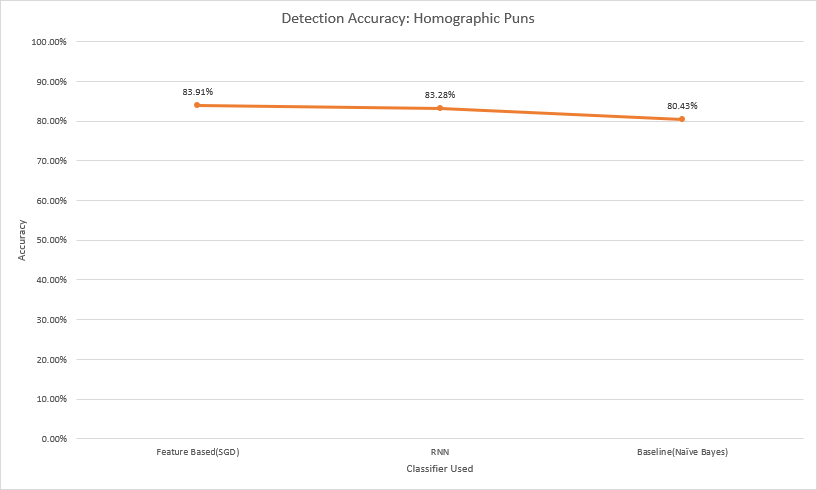
\includegraphics[width=0.85\textwidth]{HomographicDetection.png}\\
						\caption{Figure 1.1 - Pun Detection (Homographic Dataset)}
					\end{SCfigure}
					\\
					\vspace{20mm}
					\begin{SCfigure}
						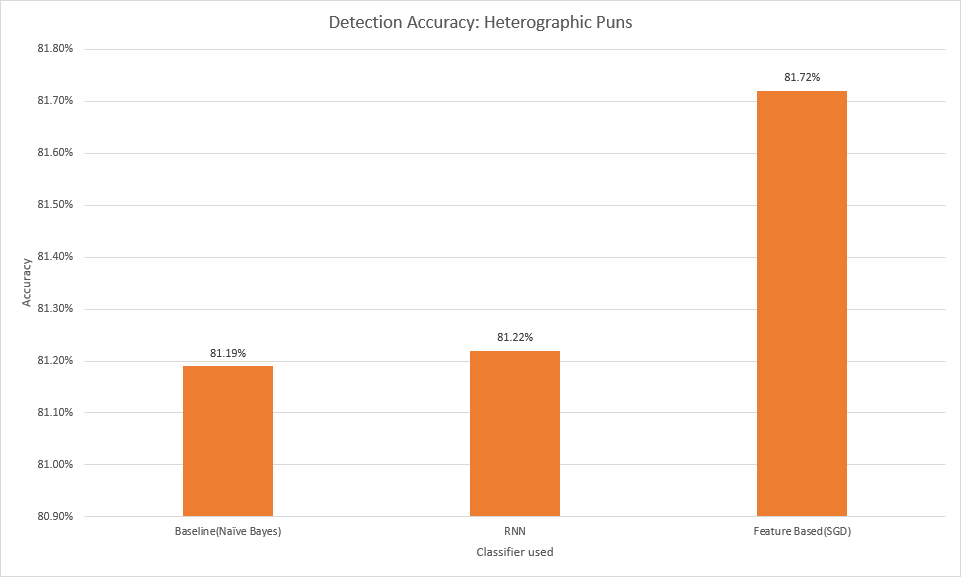
\includegraphics[width=0.85\textwidth]{HeterographicDetection.png}\\
						\caption{Figure 1.2 - Pun Detection (Heterographic Dataset)}
					\end{SCfigure}
				\end{column}
				%----------------------------------------------------------------------------------------
				% end top center column
				%----------------------------------------------------------------------------------------
			\end{columns}
			\begin{block}
				{.}
			\end{block}
			%----------------------------------------------------------------------------------------
			% bottom row
			%----------------------------------------------------------------------------------------
			\begin{columns}[t,totalwidth=\twocolwid]
				\begin{column}{15mm}\end{column}
				%----------------------------------------------------------------------------------------
				% left column
				%----------------------------------------------------------------------------------------
				\begin{column}{\onecolwid}

					\vspace{25mm}
					\begin{SCfigure}
					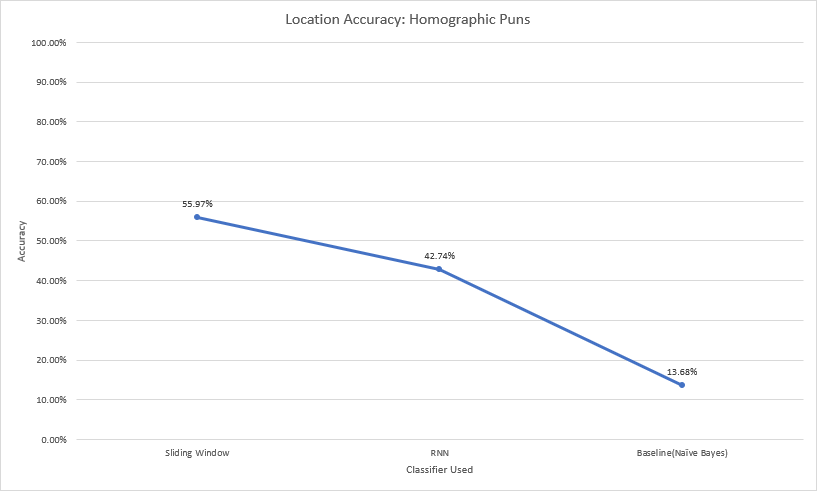
\includegraphics[width=0.85\textwidth]{HomographicLocation.png}\\
					\caption{Figure 2.1 - Pun Location (Homographic Dataset)}
					\end{SCfigure}
					\\
					\vspace{20mm}
					\begin{SCfigure}
					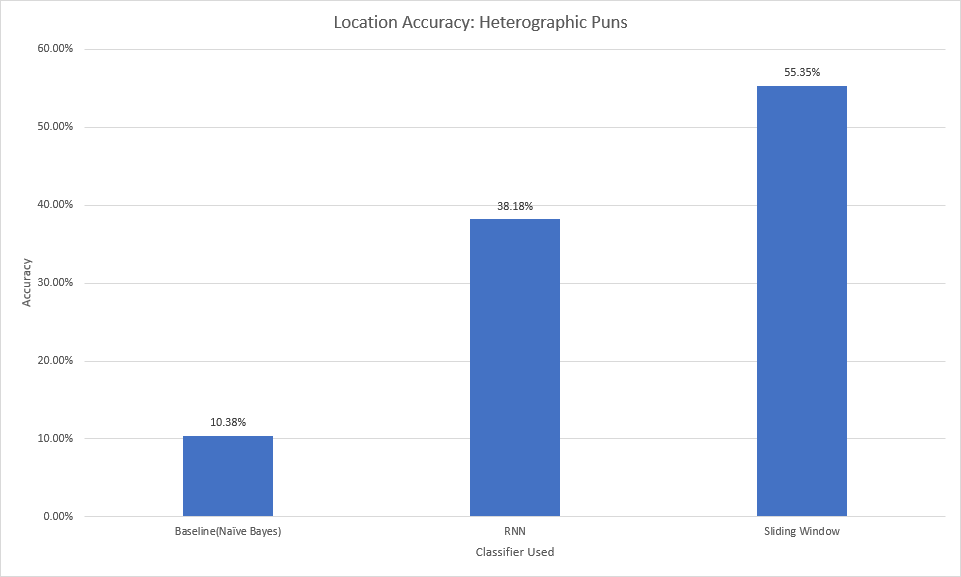
\includegraphics[width=0.85\textwidth]{HeterographicLocation.png}\\
					\caption{Figure 2.2 - Pun Location (Heterographic Dataset)}
					\end{SCfigure}
				\end{column}
				%----------------------------------------------------------------------------------------
				% right column
				%----------------------------------------------------------------------------------------
				\begin{column}{\onecolwid}
					\vspace{55mm}
					\begin{block}{Pun Location Algorithms}
						{\large 
							\begin{itemize}
								\item {\textbf{Multinomial Naive Bayes}\\
									Our baseline---an easy to implement algorithm which we measured approaches against
								}
								\item {\textbf{Sequence-Labeling Bidirectional LSTM}\\
									A Sequence-Labeling LSTM using glove embeddings for word representation.
								}
								\item {\textbf{Sliding Window MEMM}\\
									A Maximum-Entropy Markov Model for Sequence Labeling. Allows us to include an arbitrary set features. Incorporates a "window" of context into the decision made at each timestep. Uses a window-size of 5. 
								}
							\end{itemize}
							\\
						}
					\end{block}
				\end{column}
				\begin{column}{\sepwid}\end{column}
			\end{columns}
		\end{column}
		\begin{column}{\sepwid}\end{column}
		%----------------------------------------------------------------------------------------
		% rightmost column
		%----------------------------------------------------------------------------------------
		\begin{column}{\onecolwid}
            \begin{block}{Performance Comparison}
				\large{
					We compare our systems to those presented at SemEval2017, the conference which proposed these tasks.
				}
				\vspace{10mm}
				%----------------------------------------------------------------------------------------
				% Pun Detection Table
				%----------------------------------------------------------------------------------------
				\begin{center}
					\begin{tabular}{ c|c|c } 
						\multicolumn{3}{c}{\textbf{Pun Detection Accuracy}}\\
						 & Homographic & Heterographic \\ 
						\hline
						SemEval & .8533 & .7837 \\ 
						\hline
						Reword & \textbf{.8565} & \textbf{.8052} \\ 
					\end{tabular}
				\end{center}
				\vspace{10mm}
				%----------------------------------------------------------------------------------------
				% Pun Location Table
				%----------------------------------------------------------------------------------------
				\begin{center}
					\begin{tabular}{ c|c|c } 
						\multicolumn{3}{c}{\textbf{Pun Location F-1}}\\
						 & Homographic & Heterographic \\ 
						\hline
						SemEval & \textbf{.6631} & \textbf{.7954} \\ 
						\hline
						Reword & .5597 & .5535 \\ 
					\end{tabular}
				\end{center}
            \end{block}
            \vspace{20mm}
            \begin{block}{Challenges}
				\large{
					\begin{itemize}
						\item {\textbf{Data}:
							The dataset is small, making it hard to tell if our results will generalize.
						}
						\item {\textbf{Error Analysis}:
							Puns vary wildly even with a given type, making error analysis difficult.
						}
					\end{itemize}
				}
            \end{block}
            \vspace{20mm}
			\begin{block}{Application}
				\large{
					We Made a UI to display our system's guess at whether a sentence is a pun. Give it a try!
				}
				\vspace{20mm}

				\begin{SCfigure}
					\centering
					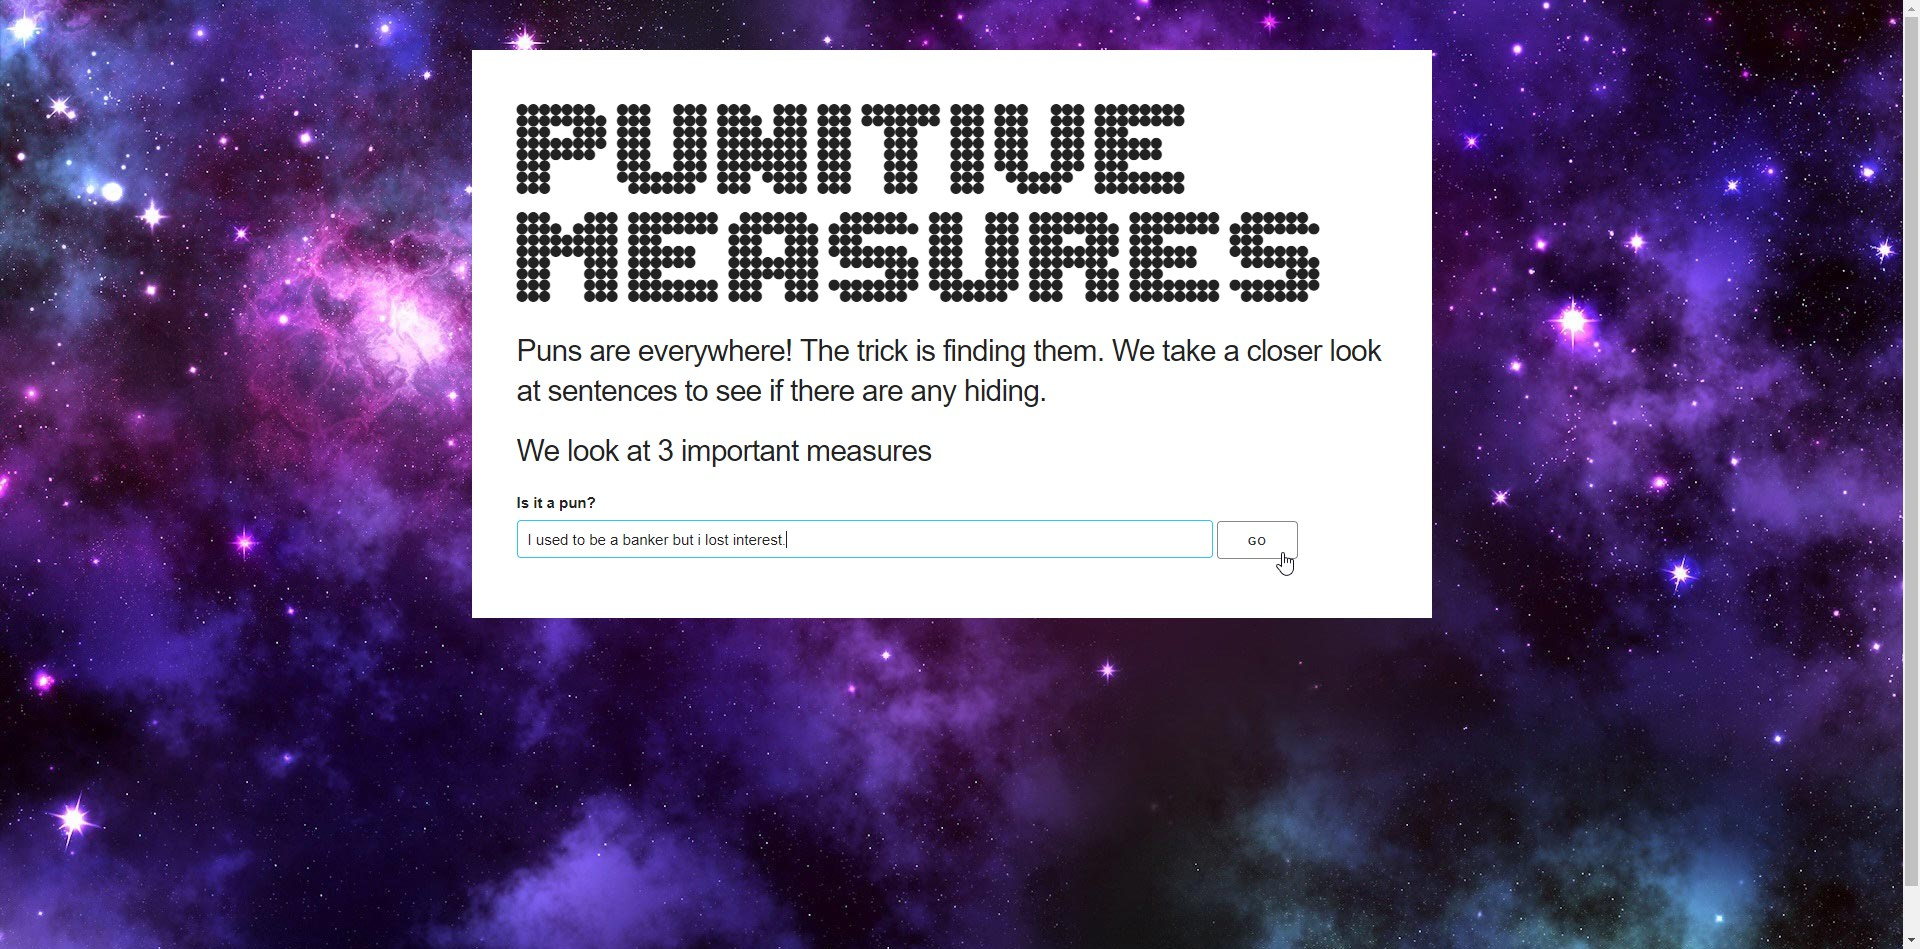
\includegraphics[width=0.75\textwidth]{UI_1.jpg}\\
				\end{SCfigure}
				\\
				\vspace{20mm}
				\begin{SCfigure}
					\centering
					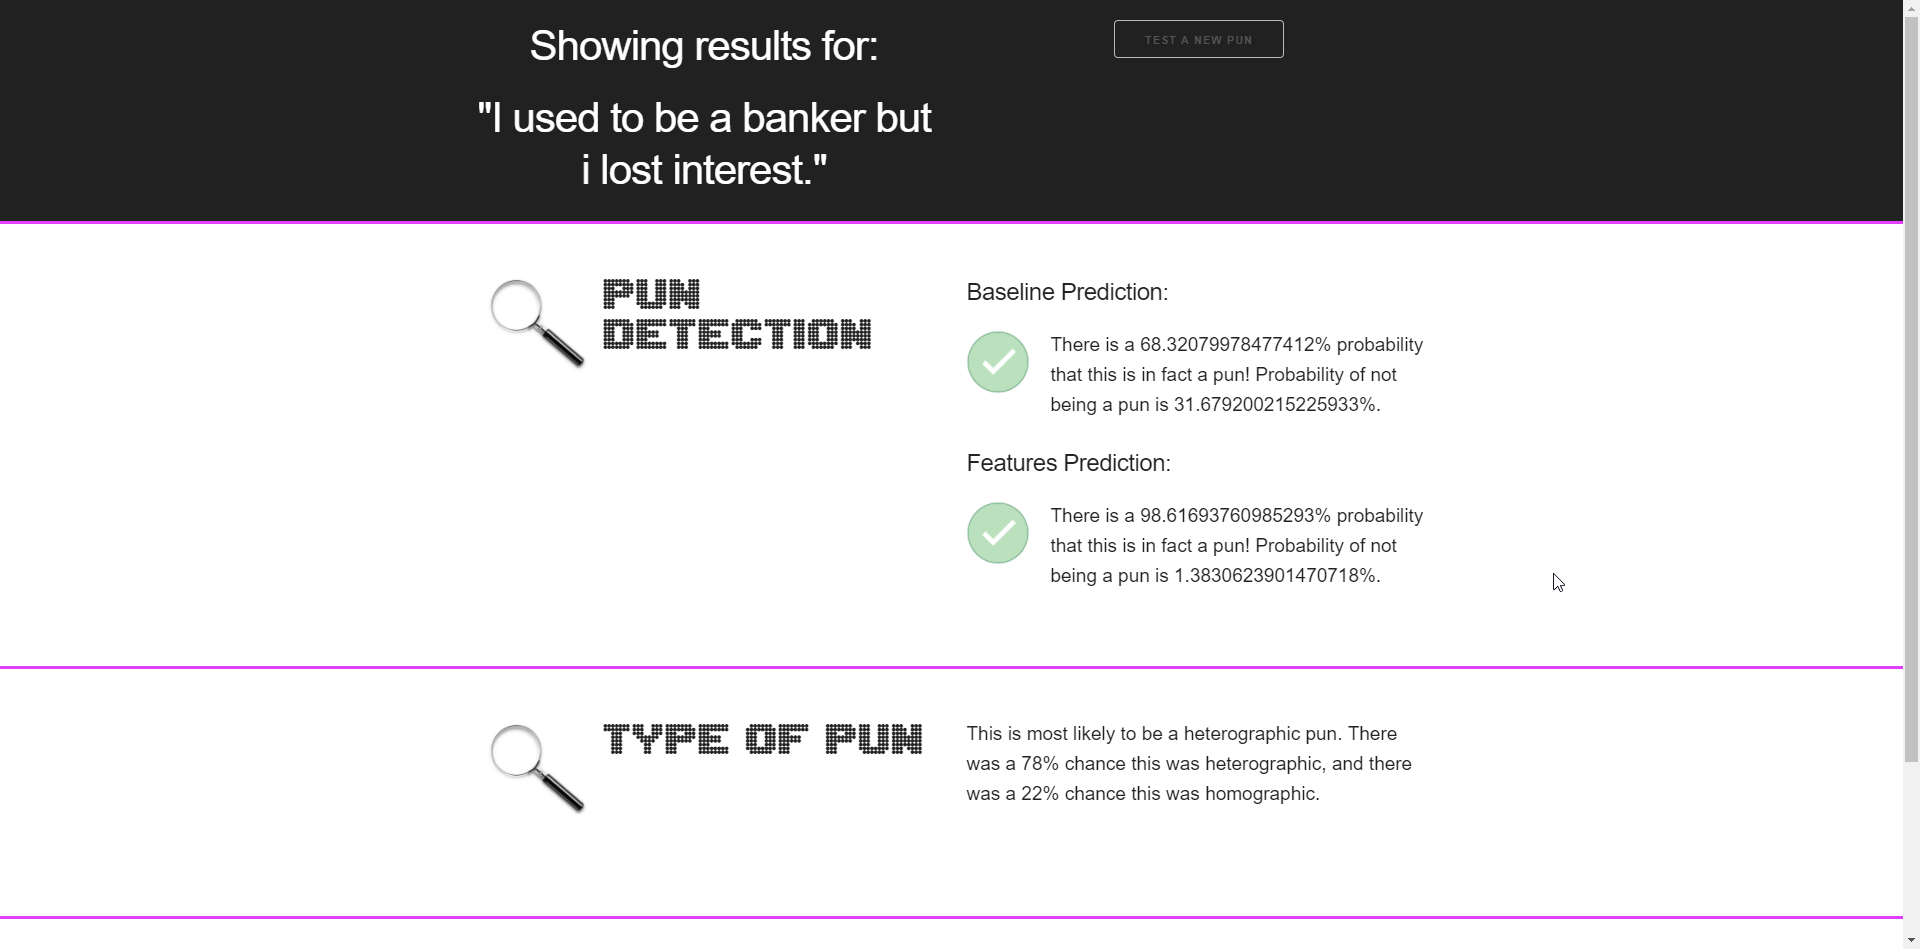
\includegraphics[width=0.75\textwidth]{UI_2.png}\\
				\end{SCfigure}
			\end{block}
			\vspace{20mm}
		\end{column}
		\begin{column}{\sepwid}\end{column}
	\end{columns}
\end{frame}
\end{document}
